\PassOptionsToPackage{unicode=true}{hyperref} % options for packages loaded elsewhere
\PassOptionsToPackage{hyphens}{url}
%
\documentclass[]{article}
\usepackage{lmodern}
\usepackage{amssymb,amsmath}
\usepackage{ifxetex,ifluatex}
\usepackage{fixltx2e} % provides \textsubscript
\ifnum 0\ifxetex 1\fi\ifluatex 1\fi=0 % if pdftex
  \usepackage[T1]{fontenc}
  \usepackage[utf8]{inputenc}
  \usepackage{textcomp} % provides euro and other symbols
\else % if luatex or xelatex
  \usepackage{unicode-math}
  \defaultfontfeatures{Ligatures=TeX,Scale=MatchLowercase}
\fi
% use upquote if available, for straight quotes in verbatim environments
\IfFileExists{upquote.sty}{\usepackage{upquote}}{}
% use microtype if available
\IfFileExists{microtype.sty}{%
\usepackage[]{microtype}
\UseMicrotypeSet[protrusion]{basicmath} % disable protrusion for tt fonts
}{}
\IfFileExists{parskip.sty}{%
\usepackage{parskip}
}{% else
\setlength{\parindent}{0pt}
\setlength{\parskip}{6pt plus 2pt minus 1pt}
}
\usepackage{hyperref}
\hypersetup{
            pdftitle={Web Scrape},
            pdfauthor={Jeff Cavanagh},
            pdfborder={0 0 0},
            breaklinks=true}
\urlstyle{same}  % don't use monospace font for urls
\usepackage[margin=1in]{geometry}
\usepackage{color}
\usepackage{fancyvrb}
\newcommand{\VerbBar}{|}
\newcommand{\VERB}{\Verb[commandchars=\\\{\}]}
\DefineVerbatimEnvironment{Highlighting}{Verbatim}{commandchars=\\\{\}}
% Add ',fontsize=\small' for more characters per line
\usepackage{framed}
\definecolor{shadecolor}{RGB}{248,248,248}
\newenvironment{Shaded}{\begin{snugshade}}{\end{snugshade}}
\newcommand{\AlertTok}[1]{\textcolor[rgb]{0.94,0.16,0.16}{#1}}
\newcommand{\AnnotationTok}[1]{\textcolor[rgb]{0.56,0.35,0.01}{\textbf{\textit{#1}}}}
\newcommand{\AttributeTok}[1]{\textcolor[rgb]{0.77,0.63,0.00}{#1}}
\newcommand{\BaseNTok}[1]{\textcolor[rgb]{0.00,0.00,0.81}{#1}}
\newcommand{\BuiltInTok}[1]{#1}
\newcommand{\CharTok}[1]{\textcolor[rgb]{0.31,0.60,0.02}{#1}}
\newcommand{\CommentTok}[1]{\textcolor[rgb]{0.56,0.35,0.01}{\textit{#1}}}
\newcommand{\CommentVarTok}[1]{\textcolor[rgb]{0.56,0.35,0.01}{\textbf{\textit{#1}}}}
\newcommand{\ConstantTok}[1]{\textcolor[rgb]{0.00,0.00,0.00}{#1}}
\newcommand{\ControlFlowTok}[1]{\textcolor[rgb]{0.13,0.29,0.53}{\textbf{#1}}}
\newcommand{\DataTypeTok}[1]{\textcolor[rgb]{0.13,0.29,0.53}{#1}}
\newcommand{\DecValTok}[1]{\textcolor[rgb]{0.00,0.00,0.81}{#1}}
\newcommand{\DocumentationTok}[1]{\textcolor[rgb]{0.56,0.35,0.01}{\textbf{\textit{#1}}}}
\newcommand{\ErrorTok}[1]{\textcolor[rgb]{0.64,0.00,0.00}{\textbf{#1}}}
\newcommand{\ExtensionTok}[1]{#1}
\newcommand{\FloatTok}[1]{\textcolor[rgb]{0.00,0.00,0.81}{#1}}
\newcommand{\FunctionTok}[1]{\textcolor[rgb]{0.00,0.00,0.00}{#1}}
\newcommand{\ImportTok}[1]{#1}
\newcommand{\InformationTok}[1]{\textcolor[rgb]{0.56,0.35,0.01}{\textbf{\textit{#1}}}}
\newcommand{\KeywordTok}[1]{\textcolor[rgb]{0.13,0.29,0.53}{\textbf{#1}}}
\newcommand{\NormalTok}[1]{#1}
\newcommand{\OperatorTok}[1]{\textcolor[rgb]{0.81,0.36,0.00}{\textbf{#1}}}
\newcommand{\OtherTok}[1]{\textcolor[rgb]{0.56,0.35,0.01}{#1}}
\newcommand{\PreprocessorTok}[1]{\textcolor[rgb]{0.56,0.35,0.01}{\textit{#1}}}
\newcommand{\RegionMarkerTok}[1]{#1}
\newcommand{\SpecialCharTok}[1]{\textcolor[rgb]{0.00,0.00,0.00}{#1}}
\newcommand{\SpecialStringTok}[1]{\textcolor[rgb]{0.31,0.60,0.02}{#1}}
\newcommand{\StringTok}[1]{\textcolor[rgb]{0.31,0.60,0.02}{#1}}
\newcommand{\VariableTok}[1]{\textcolor[rgb]{0.00,0.00,0.00}{#1}}
\newcommand{\VerbatimStringTok}[1]{\textcolor[rgb]{0.31,0.60,0.02}{#1}}
\newcommand{\WarningTok}[1]{\textcolor[rgb]{0.56,0.35,0.01}{\textbf{\textit{#1}}}}
\usepackage{graphicx,grffile}
\makeatletter
\def\maxwidth{\ifdim\Gin@nat@width>\linewidth\linewidth\else\Gin@nat@width\fi}
\def\maxheight{\ifdim\Gin@nat@height>\textheight\textheight\else\Gin@nat@height\fi}
\makeatother
% Scale images if necessary, so that they will not overflow the page
% margins by default, and it is still possible to overwrite the defaults
% using explicit options in \includegraphics[width, height, ...]{}
\setkeys{Gin}{width=\maxwidth,height=\maxheight,keepaspectratio}
\setlength{\emergencystretch}{3em}  % prevent overfull lines
\providecommand{\tightlist}{%
  \setlength{\itemsep}{0pt}\setlength{\parskip}{0pt}}
\setcounter{secnumdepth}{0}
% Redefines (sub)paragraphs to behave more like sections
\ifx\paragraph\undefined\else
\let\oldparagraph\paragraph
\renewcommand{\paragraph}[1]{\oldparagraph{#1}\mbox{}}
\fi
\ifx\subparagraph\undefined\else
\let\oldsubparagraph\subparagraph
\renewcommand{\subparagraph}[1]{\oldsubparagraph{#1}\mbox{}}
\fi

% set default figure placement to htbp
\makeatletter
\def\fps@figure{htbp}
\makeatother


\title{Web Scrape}
\author{Jeff Cavanagh}
\date{2020-08-05}

\begin{document}
\maketitle

\textbf{Unfortunately, not all data is contained within neat dataframes.
Much of the freely accessible data out there is posted on webpages. This
post will serve as an introduction on how to extract that data using two
packages: \texttt{rvest} and \texttt{rselenium}.}

\hypertarget{setup}{%
\subsubsection{Setup}\label{setup}}

\hypertarget{css-tool}{%
\paragraph{CSS Tool}\label{css-tool}}

Webpages are not written in R code. They are written in HTML and CSS. A
working knowledge of at least CSS is required to use the webscapring
packages R provides.

Luckily for us there are free CSS selector tools to pull the the CSS
links we need. I will be using the
\href{https://selectorgadget.com/}{SelectorGadget}.

\hypertarget{data}{%
\paragraph{Data}\label{data}}

The data will be practicing our techniques on is a page from IMDb that
lists 50 comic book movies that were released between 2000 and 2019,
ranked by popularity. Here was what the page data looks like:

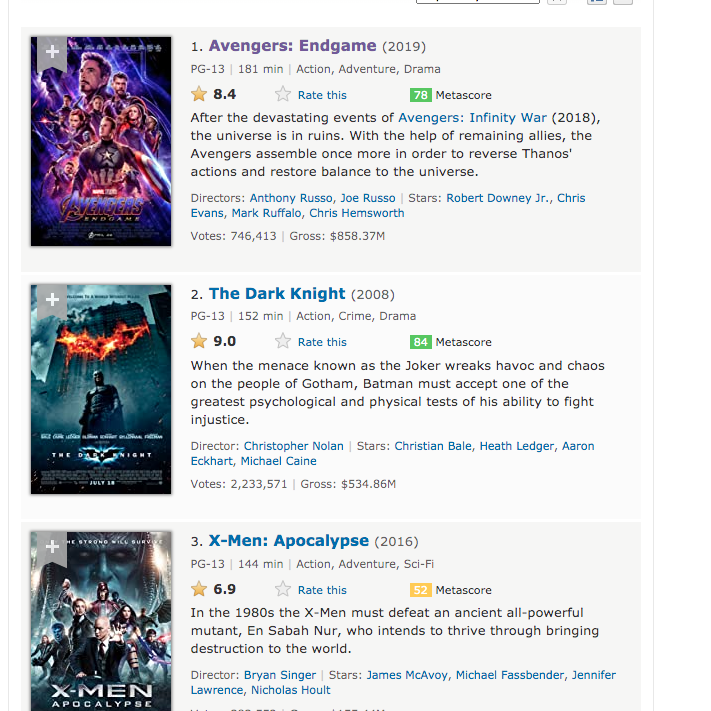
\includegraphics{/analytics/2020-08-05-web-scrape_files/Screen Shot 2020-08-08 at 2.43.03 PM.png}

The link can be found
\href{https://www.imdb.com/search/keyword/?keywords=based-on-comic-book\%2Csuperhero\&pf_rd_m=A2FGELUUNOQJNL\&pf_rd_p=a581b14c-5a82-4e29-9cf8-54f909ced9e1\&pf_rd_r=HA259SA49EFNVTHNRH2V\&pf_rd_s=center-5\&pf_rd_t=15051\&pf_rd_i=genre\&ref_=kw_ref_yr\&sort=moviemeter,asc\&mode=detail\&page=1\&title_type=movie\&release_date=2000\%2C2019}{here}.

Our primary goal will be to extract the different elements of data
displayed on this page and translate it into a dataframe that is easy to
use and manipulate. We will first do so with \texttt{rvest}.

\hypertarget{rvest}{%
\subsubsection{\texorpdfstring{\texttt{rvest}}{rvest}}\label{rvest}}

This package provides a host of functions that are designed to extract
html code. The first thing we need to do to use it is use
\texttt{read\_html} to the read the full page.

\begin{Shaded}
\begin{Highlighting}[]
\KeywordTok{library}\NormalTok{(tidyverse)}
\KeywordTok{library}\NormalTok{(rvest)}
\NormalTok{movies <-}\StringTok{ }\KeywordTok{read_html}\NormalTok{(}\StringTok{"https://www.imdb.com/search/keyword/?keywords=based-on-comic-book%2Csuperhero&pf_rd_m=A2FGELUUNOQJNL&pf_rd_p=a581b14c-5a82-4e29-9cf8-54f909ced9e1&pf_rd_r=HA259SA49EFNVTHNRH2V&pf_rd_s=center-5&pf_rd_t=15051&pf_rd_i=genre&ref_=kw_ref_yr&sort=moviemeter,asc&mode=detail&page=1&title_type=movie&release_date=2000%2C2019"}\NormalTok{)}
\end{Highlighting}
\end{Shaded}

Now that is done, we will start to extract different text elements of
the page using \texttt{html\_nodes} to identify all matches to the input
CSS tag and \texttt{html\_text} to extract the text. First let's get all
the movie titles.

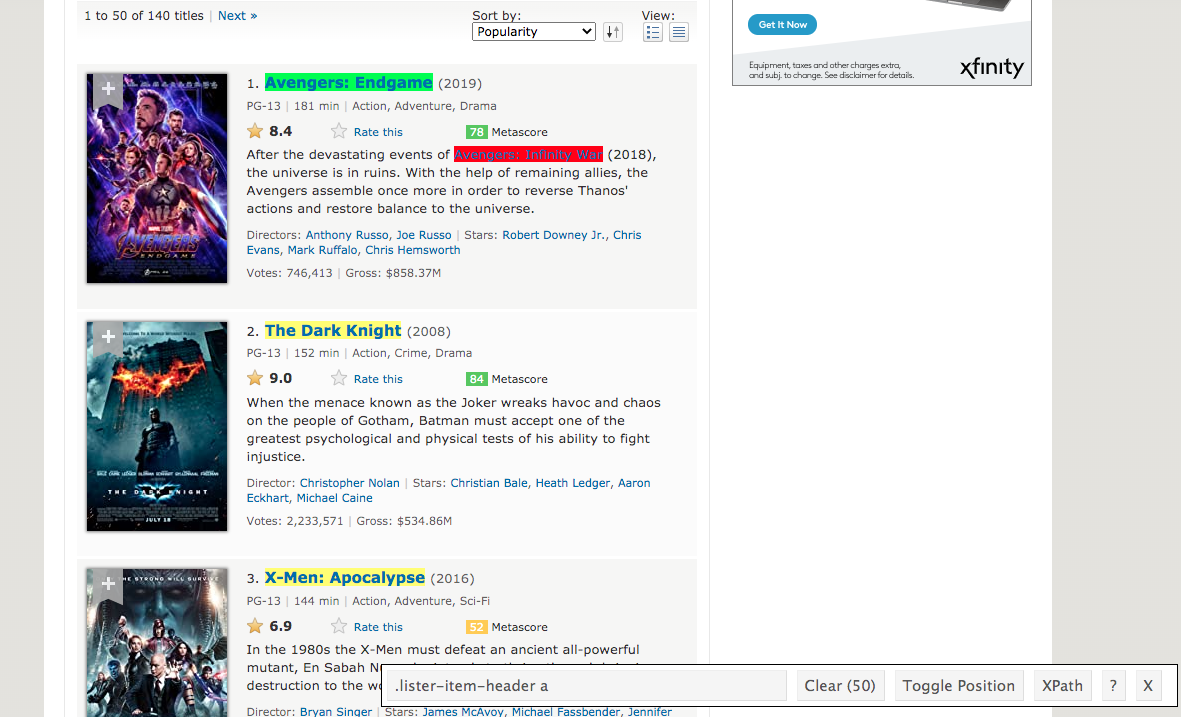
\includegraphics{/analytics/2020-08-05-web-scrape_files/Screen Shot 2020-08-08 at 12.37.06 PM.png}

\begin{Shaded}
\begin{Highlighting}[]
\NormalTok{titles <-}\StringTok{ }\NormalTok{movies }\OperatorTok
\StringTok{  }\KeywordTok{html_nodes}\NormalTok{(}\StringTok{".lister-item-header a"}\NormalTok{) }\OperatorTok
\StringTok{  }\KeywordTok{html_text}\NormalTok{()}
\end{Highlighting}
\end{Shaded}

Using the same approach we can collect the other statistics from each
movie. Let's do that now for each movies popularity ranking, rating,
IMDb rating, runtime, genre, plot, domestic gross, directors, and
actors.

\begin{Shaded}
\begin{Highlighting}[]
\NormalTok{ranking<-}\StringTok{ }\NormalTok{movies }\OperatorTok
\StringTok{  }\KeywordTok{html_nodes}\NormalTok{(}\StringTok{".text-primary"}\NormalTok{) }\OperatorTok
\StringTok{  }\KeywordTok{html_text}\NormalTok{() }\OperatorTok
\StringTok{  }\KeywordTok{as.numeric}\NormalTok{()}
\KeywordTok{head}\NormalTok{(ranking)}
\end{Highlighting}
\end{Shaded}

\begin{verbatim}
## [1] 1 2 3 4 5 6
\end{verbatim}

\begin{Shaded}
\begin{Highlighting}[]
\NormalTok{rating <-}\StringTok{ }\NormalTok{movies }\OperatorTok
\StringTok{  }\KeywordTok{html_nodes}\NormalTok{(}\StringTok{".certificate"}\NormalTok{) }\OperatorTok
\StringTok{  }\KeywordTok{html_text}\NormalTok{()}
\KeywordTok{head}\NormalTok{(rating)}
\end{Highlighting}
\end{Shaded}

\begin{verbatim}
## [1] "PG-13" "PG-13" "PG-13" "R"     "PG-13" "PG-13"
\end{verbatim}

\begin{Shaded}
\begin{Highlighting}[]
\NormalTok{IMDb_rating <-}\StringTok{ }\NormalTok{movies }\OperatorTok
\StringTok{  }\KeywordTok{html_nodes}\NormalTok{(}\StringTok{".ratings-imdb-rating strong"}\NormalTok{) }\OperatorTok
\StringTok{  }\KeywordTok{html_text}\NormalTok{() }\OperatorTok
\StringTok{  }\KeywordTok{as.numeric}\NormalTok{()}
\KeywordTok{head}\NormalTok{(IMDb_rating)}
\end{Highlighting}
\end{Shaded}

\begin{verbatim}
## [1] 8.4 9.0 6.9 7.6 7.0 8.4
\end{verbatim}

\begin{Shaded}
\begin{Highlighting}[]
\NormalTok{runtime <-}\StringTok{ }\NormalTok{movies }\OperatorTok
\StringTok{  }\KeywordTok{html_nodes}\NormalTok{(}\StringTok{".runtime"}\NormalTok{) }\OperatorTok
\StringTok{  }\KeywordTok{html_text}\NormalTok{() }\OperatorTok\StringTok{ }\CommentTok{# translating from a character string to numeric vector}
\StringTok{  }\KeywordTok{str_sub}\NormalTok{(}\DecValTok{1}\NormalTok{,}\OperatorTok{-}\DecValTok{5}\NormalTok{) }\OperatorTok
\StringTok{  }\KeywordTok{as.integer}\NormalTok{()}
\KeywordTok{head}\NormalTok{(runtime)}
\end{Highlighting}
\end{Shaded}

\begin{verbatim}
## [1] 181 152 144 162 143 149
\end{verbatim}

\begin{Shaded}
\begin{Highlighting}[]
\NormalTok{genre <-}\StringTok{ }\NormalTok{movies }\OperatorTok
\StringTok{  }\KeywordTok{html_nodes}\NormalTok{(}\StringTok{".genre"}\NormalTok{) }\OperatorTok
\StringTok{  }\KeywordTok{html_text}\NormalTok{() }\OperatorTok\StringTok{ }\CommentTok{# cleaning character string}
\StringTok{  }\KeywordTok{str_remove}\NormalTok{(}\StringTok{"^}\CharTok{\textbackslash{}\textbackslash{}}\StringTok{n"}\NormalTok{) }\OperatorTok
\StringTok{  }\KeywordTok{str_squish}\NormalTok{()}
\KeywordTok{head}\NormalTok{(genre)}
\end{Highlighting}
\end{Shaded}

\begin{verbatim}
## [1] "Action, Adventure, Drama"   "Action, Crime, Drama"      
## [3] "Action, Adventure, Sci-Fi"  "Action, Drama, Mystery"    
## [5] "Action, Adventure, Fantasy" "Action, Adventure, Sci-Fi"
\end{verbatim}

\begin{Shaded}
\begin{Highlighting}[]
\NormalTok{plot <-}\StringTok{ }\NormalTok{movies }\OperatorTok
\StringTok{  }\KeywordTok{html_nodes}\NormalTok{(}\StringTok{".ratings-bar+ p"}\NormalTok{) }\OperatorTok
\StringTok{  }\KeywordTok{html_text}\NormalTok{() }\OperatorTok\StringTok{ }\CommentTok{# cleaning up character strings}
\StringTok{  }\KeywordTok{str_remove}\NormalTok{(}\StringTok{"^}\CharTok{\textbackslash{}\textbackslash{}}\StringTok{n}\CharTok{\textbackslash{}\textbackslash{}}\StringTok{s+"}\NormalTok{)}
\KeywordTok{head}\NormalTok{(plot)}
\end{Highlighting}
\end{Shaded}

\begin{verbatim}
## [1] "After the devastating events of Avengers: Infinity War (2018), the universe is in ruins. With the help of remaining allies, the Avengers assemble once more in order to reverse Thanos' actions and restore balance to the universe."
## [2] "When the menace known as the Joker wreaks havoc and chaos on the people of Gotham, Batman must accept one of the greatest psychological and physical tests of his ability to fight injustice."                                       
## [3] "In the 1980s the X-Men must defeat an ancient all-powerful mutant, En Sabah Nur, who intends to thrive through bringing destruction to the world."                                                                                   
## [4] "In 1985 where former superheroes exist, the murder of a colleague sends active vigilante Rorschach into his own sprawling investigation, uncovering something that could completely change the course of history as we know it."     
## [5] "Arthur Curry, the human-born heir to the underwater kingdom of Atlantis, goes on a quest to prevent a war between the worlds of ocean and land."                                                                                     
## [6] "The Avengers and their allies must be willing to sacrifice all in an attempt to defeat the powerful Thanos before his blitz of devastation and ruin puts an end to the universe."
\end{verbatim}

\begin{Shaded}
\begin{Highlighting}[]
\NormalTok{gross_domestic <-}\StringTok{ }\NormalTok{movies }\OperatorTok
\StringTok{  }\KeywordTok{html_nodes}\NormalTok{(}\StringTok{".ghost~ .text-muted+ span"}\NormalTok{) }\OperatorTok
\StringTok{  }\KeywordTok{html_text}\NormalTok{() }\OperatorTok\StringTok{ }\CommentTok{# translating from a character string into a numeric vector}
\StringTok{  }\KeywordTok{str_remove_all}\NormalTok{(}\StringTok{"^}\CharTok{\textbackslash{}\textbackslash{}}\StringTok{$|M$"}\NormalTok{) }\OperatorTok\StringTok{ }\CommentTok{# all of our entries are in millions so easy to convert}
\StringTok{  }\KeywordTok{as.numeric}\NormalTok{() }\OperatorTok{*}\StringTok{ }\FloatTok{1e6}
\KeywordTok{head}\NormalTok{(gross_domestic)}
\end{Highlighting}
\end{Shaded}

\begin{verbatim}
## [1] 858370000 534860000 155440000 107510000 335060000 678820000
\end{verbatim}

\begin{Shaded}
\begin{Highlighting}[]
\NormalTok{directors1 <-}\StringTok{ }\NormalTok{movies }\OperatorTok
\StringTok{  }\KeywordTok{html_nodes}\NormalTok{(}\StringTok{".text-small a:nth-child(1)"}\NormalTok{) }\OperatorTok
\StringTok{  }\KeywordTok{html_text}\NormalTok{()}
\KeywordTok{head}\NormalTok{(directors1)}
\end{Highlighting}
\end{Shaded}

\begin{verbatim}
## [1] "Anthony Russo"     "Christopher Nolan" "Bryan Singer"     
## [4] "Zack Snyder"       "James Wan"         "Anthony Russo"
\end{verbatim}

\begin{Shaded}
\begin{Highlighting}[]
\KeywordTok{length}\NormalTok{(directors1)}
\end{Highlighting}
\end{Shaded}

\begin{verbatim}
## [1] 50
\end{verbatim}

\begin{Shaded}
\begin{Highlighting}[]
\NormalTok{directors2 <-}\StringTok{ }\NormalTok{movies }\OperatorTok
\StringTok{  }\KeywordTok{html_nodes}\NormalTok{(}\StringTok{".text-small a:nth-child(1) , .text-small a:nth-child(2)"}\NormalTok{) }\OperatorTok
\StringTok{  }\KeywordTok{html_text}\NormalTok{()}
\KeywordTok{head}\NormalTok{(directors2)}
\end{Highlighting}
\end{Shaded}

\begin{verbatim}
## [1] "Anthony Russo"     "Joe Russo"         "Christopher Nolan"
## [4] "Bryan Singer"      "Zack Snyder"       "James Wan"
\end{verbatim}

\begin{Shaded}
\begin{Highlighting}[]
\KeywordTok{length}\NormalTok{(directors2)}
\end{Highlighting}
\end{Shaded}

\begin{verbatim}
## [1] 57
\end{verbatim}

\begin{Shaded}
\begin{Highlighting}[]
\NormalTok{actors1 <-}\StringTok{ }\NormalTok{movies }\OperatorTok
\StringTok{  }\KeywordTok{html_nodes}\NormalTok{(}\StringTok{".text-small .ghost+ a"}\NormalTok{) }\OperatorTok
\StringTok{  }\KeywordTok{html_text}\NormalTok{()}
\KeywordTok{head}\NormalTok{(actors1)}
\end{Highlighting}
\end{Shaded}

\begin{verbatim}
## [1] "Robert Downey Jr."  "Christian Bale"     "James McAvoy"      
## [4] "Jackie Earle Haley" "Jason Momoa"        "Robert Downey Jr."
\end{verbatim}

\begin{Shaded}
\begin{Highlighting}[]
\KeywordTok{length}\NormalTok{(actors1)}
\end{Highlighting}
\end{Shaded}

\begin{verbatim}
## [1] 50
\end{verbatim}

\begin{Shaded}
\begin{Highlighting}[]
\NormalTok{actors2 <-}\StringTok{ }\NormalTok{movies }\OperatorTok
\StringTok{  }\KeywordTok{html_nodes}\NormalTok{(}\StringTok{".text-small .ghost~ a"}\NormalTok{) }\OperatorTok
\StringTok{  }\KeywordTok{html_text}\NormalTok{()}
\KeywordTok{head}\NormalTok{(actors2)}
\end{Highlighting}
\end{Shaded}

\begin{verbatim}
## [1] "Robert Downey Jr." "Chris Evans"       "Mark Ruffalo"     
## [4] "Chris Hemsworth"   "Christian Bale"    "Heath Ledger"
\end{verbatim}

\begin{Shaded}
\begin{Highlighting}[]
\KeywordTok{length}\NormalTok{(actors2)}
\end{Highlighting}
\end{Shaded}

\begin{verbatim}
## [1] 200
\end{verbatim}

For the most part we cleaned each vector we compiled as we extracted the
data. Take note of the actor and director variables though.
\texttt{director1} and \texttt{actor1} each have a length of 50
(matching the rest of the data). \texttt{director2} and \texttt{actor2}
have more entries though, because all the movies on the list have more
than one actor, and some have multiple directors.

To rectify this we will combine concatentate these strings with
\texttt{str\_c} using \texttt{for} loops. To do this, we will index the
directors by appearance in the \texttt{directors1} and by taking
groupings of four actors (as four actors are listed for each movie).

\begin{Shaded}
\begin{Highlighting}[]
\NormalTok{ind <-}\StringTok{ }\KeywordTok{which}\NormalTok{(directors2 }\OperatorTok\StringTok{ }\NormalTok{directors1) }\OperatorTok\StringTok{ }\KeywordTok{append}\NormalTok{(}\KeywordTok{length}\NormalTok{(directors2)}\OperatorTok{+}\DecValTok{1}\NormalTok{)}
\NormalTok{directors <-}\StringTok{ }\KeywordTok{c}\NormalTok{()}
\ControlFlowTok{for}\NormalTok{ (i }\ControlFlowTok{in} \DecValTok{1}\OperatorTok{:}\NormalTok{(}\KeywordTok{length}\NormalTok{(ind)}\OperatorTok{-}\DecValTok{1}\NormalTok{))\{}
\NormalTok{  directors[i] <-}\StringTok{ }\KeywordTok{str_c}\NormalTok{(directors2[}\KeywordTok{c}\NormalTok{(ind[i]}\OperatorTok{:}\NormalTok{(ind[i}\OperatorTok{+}\DecValTok{1}\NormalTok{]}\OperatorTok{-}\DecValTok{1}\NormalTok{))], }\DataTypeTok{collapse =} \StringTok{", "}\NormalTok{)}
\NormalTok{\}}
\KeywordTok{head}\NormalTok{(directors)}
\end{Highlighting}
\end{Shaded}

\begin{verbatim}
## [1] "Anthony Russo, Joe Russo" "Christopher Nolan"       
## [3] "Bryan Singer"             "Zack Snyder"             
## [5] "James Wan"                "Anthony Russo, Joe Russo"
\end{verbatim}

\begin{Shaded}
\begin{Highlighting}[]
\NormalTok{actors <-}\StringTok{ }\KeywordTok{c}\NormalTok{()}
\ControlFlowTok{for}\NormalTok{(i }\ControlFlowTok{in} \DecValTok{1}\OperatorTok{:}\KeywordTok{length}\NormalTok{(actors1))\{}
\NormalTok{  actors[i] <-}\StringTok{ }\KeywordTok{str_c}\NormalTok{(actors2[}\KeywordTok{c}\NormalTok{(((i}\DecValTok{-1}\NormalTok{) }\OperatorTok{*}\StringTok{ }\DecValTok{4} \OperatorTok{+}\StringTok{ }\DecValTok{1}\NormalTok{)}\OperatorTok{:}\NormalTok{(}\DecValTok{4} \OperatorTok{*}\StringTok{ }\NormalTok{i))], }\DataTypeTok{collapse =} \StringTok{", "}\NormalTok{)}
\NormalTok{\}}
\KeywordTok{head}\NormalTok{(actors)}
\end{Highlighting}
\end{Shaded}

\begin{verbatim}
## [1] "Robert Downey Jr., Chris Evans, Mark Ruffalo, Chris Hemsworth"      
## [2] "Christian Bale, Heath Ledger, Aaron Eckhart, Michael Caine"         
## [3] "James McAvoy, Michael Fassbender, Jennifer Lawrence, Nicholas Hoult"
## [4] "Jackie Earle Haley, Patrick Wilson, Carla Gugino, Malin Akerman"    
## [5] "Jason Momoa, Amber Heard, Willem Dafoe, Patrick Wilson"             
## [6] "Robert Downey Jr., Chris Hemsworth, Mark Ruffalo, Chris Evans"
\end{verbatim}

We now have most of the primary data we were searching for. Now lets
combine it into a functioning data frame.

\begin{Shaded}
\begin{Highlighting}[]
\NormalTok{superhero_movies <-}\StringTok{ }\KeywordTok{tibble}\NormalTok{(}
\NormalTok{  titles,}
  \DataTypeTok{popularity_rank =}\NormalTok{ ranking,}
\NormalTok{  IMDb_rating,}
\NormalTok{  rating,}
\NormalTok{  runtime,}
\NormalTok{  genre,}
\NormalTok{  gross_domestic,}
\NormalTok{  plot,}
\NormalTok{  directors,}
\NormalTok{  actors}
\NormalTok{)}
\KeywordTok{str}\NormalTok{(superhero_movies)}
\end{Highlighting}
\end{Shaded}

\begin{verbatim}
## tibble [50 x 10] (S3: tbl_df/tbl/data.frame)
##  $ titles         : chr [1:50] "Avengers: Endgame" "The Dark Knight" "X-Men: Apocalypse" "Watchmen" ...
##  $ popularity_rank: num [1:50] 1 2 3 4 5 6 7 8 9 10 ...
##  $ IMDb_rating    : num [1:50] 8.4 9 6.9 7.6 7 8.4 8.4 6.3 8 7.6 ...
##  $ rating         : chr [1:50] "PG-13" "PG-13" "PG-13" "R" ...
##  $ runtime        : int [1:50] 181 152 144 162 143 149 164 120 121 136 ...
##  $ genre          : chr [1:50] "Action, Adventure, Drama" "Action, Crime, Drama" "Action, Adventure, Sci-Fi" "Action, Drama, Mystery" ...
##  $ gross_domestic : num [1:50] 8.58e+08 5.35e+08 1.55e+08 1.08e+08 3.35e+08 ...
##  $ plot           : chr [1:50] "After the devastating events of Avengers: Infinity War (2018), the universe is in ruins. With the help of remai"| __truncated__ "When the menace known as the Joker wreaks havoc and chaos on the people of Gotham, Batman must accept one of th"| __truncated__ "In the 1980s the X-Men must defeat an ancient all-powerful mutant, En Sabah Nur, who intends to thrive through "| __truncated__ "In 1985 where former superheroes exist, the murder of a colleague sends active vigilante Rorschach into his own"| __truncated__ ...
##  $ directors      : chr [1:50] "Anthony Russo, Joe Russo" "Christopher Nolan" "Bryan Singer" "Zack Snyder" ...
##  $ actors         : chr [1:50] "Robert Downey Jr., Chris Evans, Mark Ruffalo, Chris Hemsworth" "Christian Bale, Heath Ledger, Aaron Eckhart, Michael Caine" "James McAvoy, Michael Fassbender, Jennifer Lawrence, Nicholas Hoult" "Jackie Earle Haley, Patrick Wilson, Carla Gugino, Malin Akerman" ...
\end{verbatim}

There is one more feauture of \texttt{rvest} I would like to illustrate
before we close out this tutorial, and that is how to extract links.

We will add one more column to our new data frame that gives the link to
each movie's page using \texttt{html\_attr}. All we need to do is add
one more input, ``href'', which tells the function we want the link, not
the text of the CSS tag element.

\begin{Shaded}
\begin{Highlighting}[]
\NormalTok{pages <-}\StringTok{ }\NormalTok{movies }\OperatorTok
\StringTok{  }\KeywordTok{html_nodes}\NormalTok{(}\StringTok{".lister-item-header a"}\NormalTok{) }\OperatorTok
\StringTok{  }\KeywordTok{html_attr}\NormalTok{(}\StringTok{"href"}\NormalTok{)}
\KeywordTok{head}\NormalTok{(pages)}
\end{Highlighting}
\end{Shaded}

\begin{verbatim}
## [1] "/title/tt4154796/?ref_=kw_li_tt" "/title/tt0468569/?ref_=kw_li_tt"
## [3] "/title/tt3385516/?ref_=kw_li_tt" "/title/tt0409459/?ref_=kw_li_tt"
## [5] "/title/tt1477834/?ref_=kw_li_tt" "/title/tt4154756/?ref_=kw_li_tt"
\end{verbatim}

This now gives us the addres's within the main website, to get the full
urls all we have to do is add the main site address to the start of each
string.

\begin{Shaded}
\begin{Highlighting}[]
\NormalTok{pages <-}\StringTok{ }\KeywordTok{str_c}\NormalTok{(}\StringTok{"https://www.imdb.com"}\NormalTok{, pages)}

\NormalTok{superhero_movies <-}\StringTok{ }\KeywordTok{cbind}\NormalTok{(superhero_movies, pages)}
\NormalTok{superhero_movies }\OperatorTok\StringTok{ }\KeywordTok{head}\NormalTok{()}
\end{Highlighting}
\end{Shaded}

\begin{verbatim}
##                   titles popularity_rank IMDb_rating rating runtime
## 1      Avengers: Endgame               1         8.4  PG-13     181
## 2        The Dark Knight               2         9.0  PG-13     152
## 3      X-Men: Apocalypse               3         6.9  PG-13     144
## 4               Watchmen               4         7.6      R     162
## 5                Aquaman               5         7.0  PG-13     143
## 6 Avengers: Infinity War               6         8.4  PG-13     149
##                        genre gross_domestic
## 1   Action, Adventure, Drama      858370000
## 2       Action, Crime, Drama      534860000
## 3  Action, Adventure, Sci-Fi      155440000
## 4     Action, Drama, Mystery      107510000
## 5 Action, Adventure, Fantasy      335060000
## 6  Action, Adventure, Sci-Fi      678820000
##                                                                                                                                                                                                                                   plot
## 1 After the devastating events of Avengers: Infinity War (2018), the universe is in ruins. With the help of remaining allies, the Avengers assemble once more in order to reverse Thanos' actions and restore balance to the universe.
## 2                                        When the menace known as the Joker wreaks havoc and chaos on the people of Gotham, Batman must accept one of the greatest psychological and physical tests of his ability to fight injustice.
## 3                                                                                    In the 1980s the X-Men must defeat an ancient all-powerful mutant, En Sabah Nur, who intends to thrive through bringing destruction to the world.
## 4      In 1985 where former superheroes exist, the murder of a colleague sends active vigilante Rorschach into his own sprawling investigation, uncovering something that could completely change the course of history as we know it.
## 5                                                                                      Arthur Curry, the human-born heir to the underwater kingdom of Atlantis, goes on a quest to prevent a war between the worlds of ocean and land.
## 6                                                     The Avengers and their allies must be willing to sacrifice all in an attempt to defeat the powerful Thanos before his blitz of devastation and ruin puts an end to the universe.
##                  directors
## 1 Anthony Russo, Joe Russo
## 2        Christopher Nolan
## 3             Bryan Singer
## 4              Zack Snyder
## 5                James Wan
## 6 Anthony Russo, Joe Russo
##                                                                actors
## 1       Robert Downey Jr., Chris Evans, Mark Ruffalo, Chris Hemsworth
## 2          Christian Bale, Heath Ledger, Aaron Eckhart, Michael Caine
## 3 James McAvoy, Michael Fassbender, Jennifer Lawrence, Nicholas Hoult
## 4     Jackie Earle Haley, Patrick Wilson, Carla Gugino, Malin Akerman
## 5              Jason Momoa, Amber Heard, Willem Dafoe, Patrick Wilson
## 6       Robert Downey Jr., Chris Hemsworth, Mark Ruffalo, Chris Evans
##                                                 pages
## 1 https://www.imdb.com/title/tt4154796/?ref_=kw_li_tt
## 2 https://www.imdb.com/title/tt0468569/?ref_=kw_li_tt
## 3 https://www.imdb.com/title/tt3385516/?ref_=kw_li_tt
## 4 https://www.imdb.com/title/tt0409459/?ref_=kw_li_tt
## 5 https://www.imdb.com/title/tt1477834/?ref_=kw_li_tt
## 6 https://www.imdb.com/title/tt4154756/?ref_=kw_li_tt
\end{verbatim}

And viola! We have taken the contents of a webpage and turned it into a
useful dataframe tracking superhero movies and all of their attached
statistics.

\hypertarget{rselenium}{%
\subsubsection{\texorpdfstring{\texttt{rselenium}}{rselenium}}\label{rselenium}}

\end{document}
